\documentclass[UTF8]{ctexart}
\usepackage{geometry}
\usepackage[backend=biber, style=authoryear]{biblatex} % 示例配置
\addbibresource{references.bib} % 替换为你的参考文献文件
\geometry{margin=1.5cm, vmargin={0pt,1cm}}
\setlength{\topmargin}{-1cm}
\setlength{\paperheight}{29.7cm}
\setlength{\textheight}{25.3cm}

% useful packages.
\usepackage{amsfonts}
\usepackage{amsmath}
\usepackage{amssymb}
\usepackage{amsthm}
\usepackage{enumerate}
\usepackage{graphicx}
\usepackage{multicol}
\usepackage{fancyhdr}
\usepackage{layout}
\usepackage{listings}
\usepackage{xcolor}
\usepackage{multirow}
\lstset{language=C++}
\setlength{\headheight}{13pt}  % 增加头部高度
\usepackage{float, caption}

% Listings setting for code formatting
\lstset{
    basicstyle=\ttfamily,
    keywordstyle=\color{blue},
    commentstyle=\color{gray},
    stringstyle=\color{red},
    breaklines=true,
    frame=single,
    numbers=left,
    numberstyle=\tiny,
    stepnumber=1,
    tabsize=4
}

% some common commands
\newcommand{\dif}{\mathrm{d}}
\newcommand{\avg}[1]{\left\langle #1 \right\rangle}
\newcommand{\difFrac}[2]{\frac{\dif #1}{\dif #2}}
\newcommand{\pdfFrac}[2]{\frac{\partial #1}{\partial #2}}
\newcommand{\OFL}{\mathrm{OFL}}
\newcommand{\UFL}{\mathrm{UFL}}
\newcommand{\fl}{\mathrm{fl}}
\newcommand{\op}{\odot}
\newcommand{\Eabs}{E_{\mathrm{abs}}}
\newcommand{\Erel}{E_{\mathrm{rel}}}

\begin{document}

\pagestyle{fancy}
\fancyhead{}
\lhead{陈梓锐}
\chead{22435036}
\rhead{\today}


%\begin{abstract}
 %   The abstract is not necessary for the theoretical homework, 
   % but for the programming project, 
    %you are encouraged to write one.      
%\end{abstract}

% ============================================
\section*{理论作业}
\subsection*{Exercise 12.11}
$u_t = vu_{xx}\ \in \omega := (0,1)\times(0,T)$
\begin{equation}
    \begin{aligned}
        \frac{U_i^{n+1}-U_i^n}{k} &= \frac{1}{2}(f(U_i^n, t_n)+f(U_i^{n+1},t_{n+1})) \\
                                  &= \frac{v}{2h^2}(U^n_{i-1} - 2U_i^n + U^n_{i+1}
                                                  + U_{i-1}^{n+1} - 2U_i^{n+1} + U_{i+1}^{n+1})
    \end{aligned}
\end{equation}
\begin{equation}
    \begin{aligned}
        \Rightarrow U_i^{n+1} - \frac{kv}{2h^2}(U^{n+1}_{i-1} - 2U_i^{n+1} + U_{i+1}^{n+1}) 
                 &= U_i^n + \frac{kv}{2h^2}(U^n_{i-1} - 2U_i^n + U^n_{i+1}) \\
                 (1 - \frac{k}{2}A)U^{n+1} &= (1 + \frac{k}{2}A)U^n + b^n
    \end{aligned}
\end{equation}
其中$U^n = (U_1^n, U_2^n, \cdots, U_m^n)^T, b^n = \frac{r}{2}(g_0(t_n)+g_0(t_{n+1}), 0, \cdots, 0, g_1(t_n)+g_1(t_{n+1}))^T$.

\subsection*{Exercise 12.26}
将空间离散化，得到ODE系统$\frac{du}{dt} = Au, A=\frac{v}{h^2}D$,$\theta$-离散公式$\frac{U^{n+1}-U^n}{k} = \theta\lambda U^{n+1} + (1-\theta)\lambda U^n$,
令$z=k\lambda$，有$U^{n+1} = \frac{1 + (1-\theta)z}{1-\theta z}U^n$.

令$R(z) = \frac{1+(1-\theta)z}{1-\theta z}, |R(z)|\leq 1, z\in \mathbb{R}^{-}$,则
\begin{equation}
    \begin{aligned}
        (\frac{1+(1-\theta)z}{1-\theta z})^2 \leq 1 &\Rightarrow (1+(1-\theta)z)^2 \leq (1-\theta z)^2 \\
                                                    &\Rightarrow 1 + 2(1-\theta)z + (1-\theta)^2z^2 \leq 1 - 2\theta z + \theta^2z^2 \\
                                                    &\Rightarrow 2z + z^2 -2\theta z^2 \leq 0 \\
                                                    &\Rightarrow (1 - 2\theta )z^2 \leq -2z
    \end{aligned}
\end{equation}
\begin{enumerate}
    \item 若$\theta \in [\frac{1}{2}, 1], (1-2\theta)z^2 \leq 0 \leq -2z$,此时方法A-stable,故$\theta$-method无条件稳定。
    \item 若$\theta \in [0, \frac{1}{2}] ,(1 - 2\theta )z^2 \leq -2z\Rightarrow z \geq \frac{-2}{1-2\theta}$,
          因为$\lambda \geq -\frac{4v}{h^2}$,所以$k \leq \frac{h^2}{2v(1-2\theta)}$时MOL方法稳定。
\end{enumerate}

\section*{编程作业}
\subsection*{如何使用}
在code中build文件下使用make命令编译，编译成功后，在build文件夹下会生成可执行文件main,在test目录下的main.json调整初始条件即可使用不同的测试用例。

在文件EquationSolverFactory.h中，设计了工厂模式以及单例模式，为选择不同的求解器提供了方便。
\begin{lstlisting}[language=C++]
{
    "method" : "Col10",
    "output_file" : "output",
    "r" : 0.5,
    "is_exact": false,
    "time" : 10
}
\end{lstlisting}

\begin{enumerate}
    \item method选择不同的方法与精度
    \item r选择不同的r值
    \item is\_exact选择是否进行精确解测试
    \item time选择测试次数
\end{enumerate}
注意只有选择用精确解测试时才需选择time，若不用精确解测试只需在method后输入迭代次数即可。
在我的函数中，h被固定为$\frac{1}{20}$,若要使用$r = \frac{1}{2h}$，只需将r设置为0即可。

可供选择的求解器有：
\begin{enumerate}
    \item \textbf{CN}：Crank-Nicolson
    \item \textbf{BE}：BTCS
    \item \textbf{Col}：collocation method
    \item \textbf{FE}：FTCS
\end{enumerate}

\subsection*{结果展示}
以下只展示了Example 12.39中的结果，其他测试均可通过更改json文件进行测试。
\textbf{真解}
\begin{figure}[H]
    \centering
    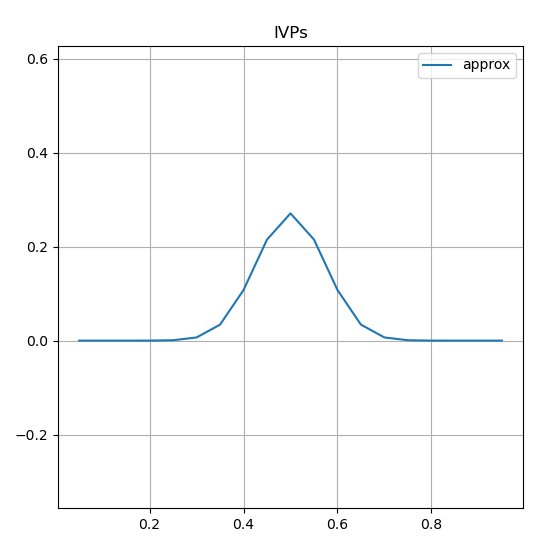
\includegraphics[width=0.2\textwidth]{exact1.png}
    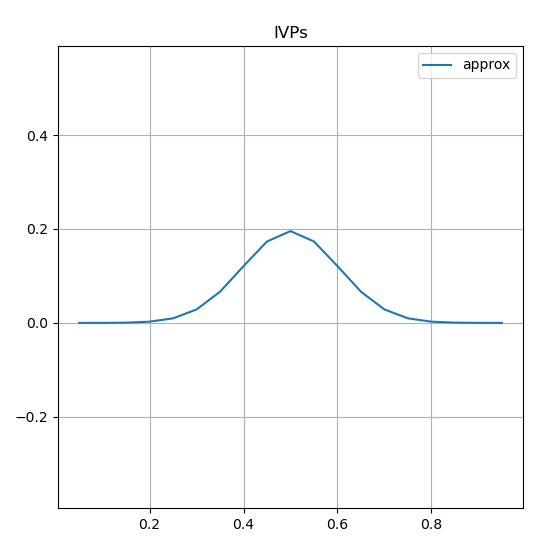
\includegraphics[width=0.2\textwidth]{exact2.png}
    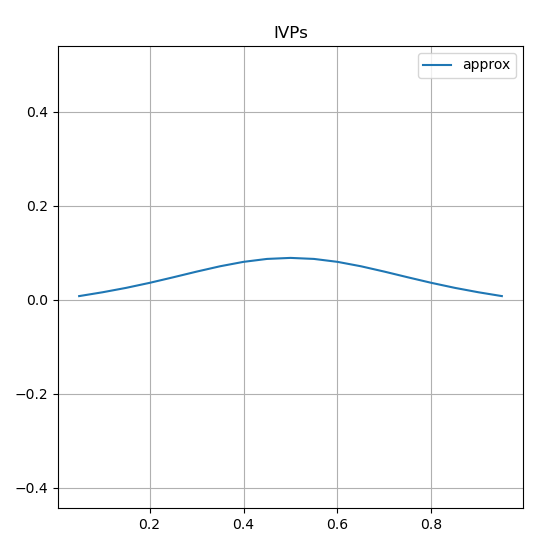
\includegraphics[width=0.2\textwidth]{exact10.png}
    \caption{exact solution}
\end{figure}

\textbf{Crank-Nicolson with r = 1}
\begin{figure}[H]
    \centering
    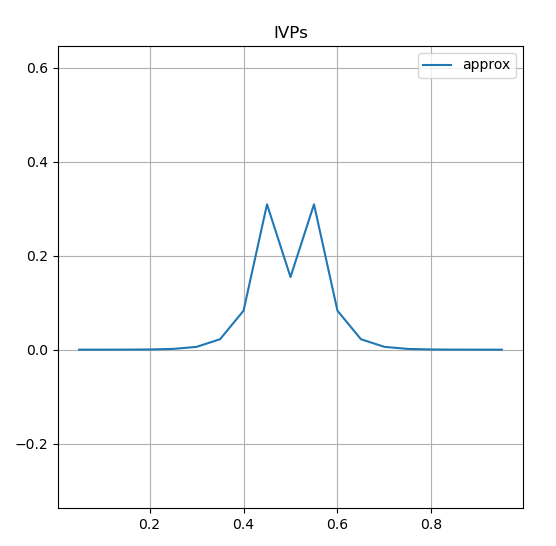
\includegraphics[width=0.2\textwidth]{CN11.png}
    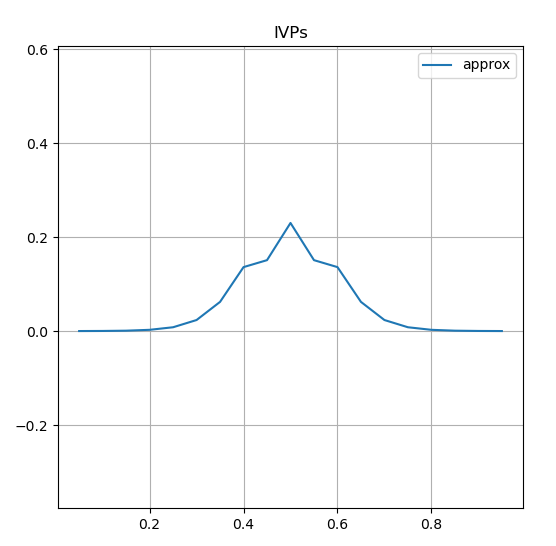
\includegraphics[width=0.2\textwidth]{CN12.png}
    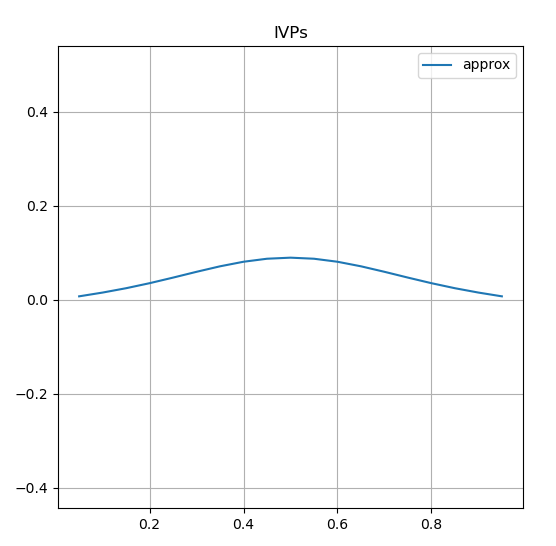
\includegraphics[width=0.2\textwidth]{CN110.png}
    \caption{Crank-Nicolson with r = 1}
\end{figure}

\textbf{Crank-Nicolson with r = 2}
\begin{figure}[H]
    \centering
    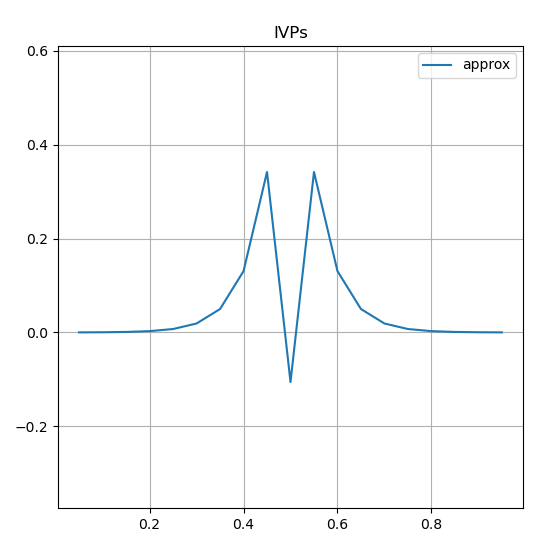
\includegraphics[width=0.2\textwidth]{CN21.png}
    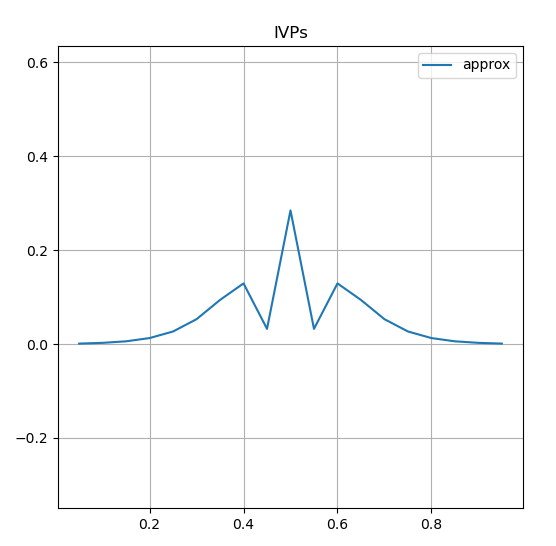
\includegraphics[width=0.2\textwidth]{CN22.png}
    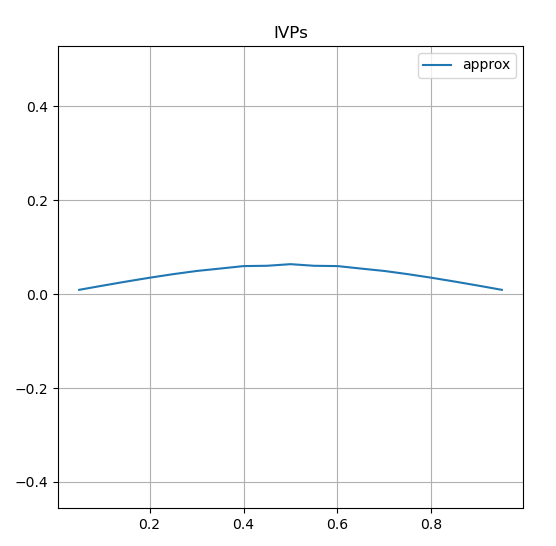
\includegraphics[width=0.2\textwidth]{CN210.png}
    \caption{Crank-Nicolson with r = 2}
\end{figure}

\textbf{BTCS method}
\begin{figure}[H]
    \centering
    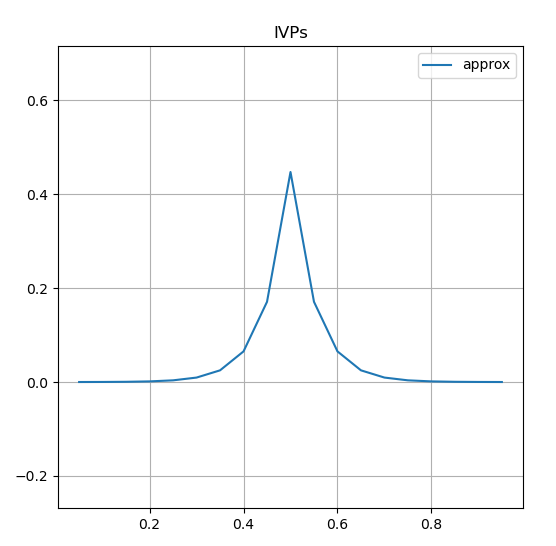
\includegraphics[width=0.2\textwidth]{BE1.png}
    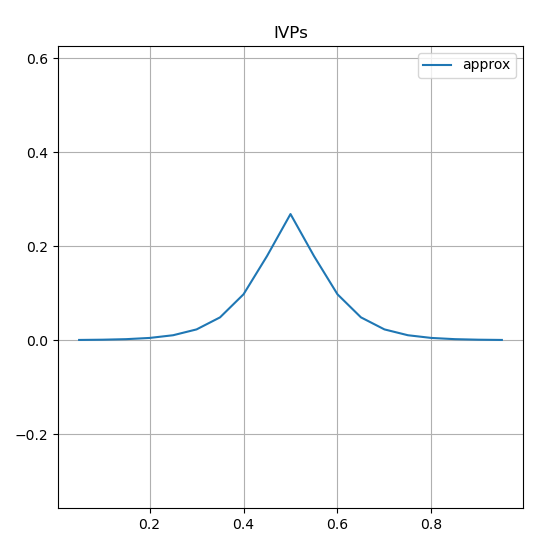
\includegraphics[width=0.2\textwidth]{BE2.png}
    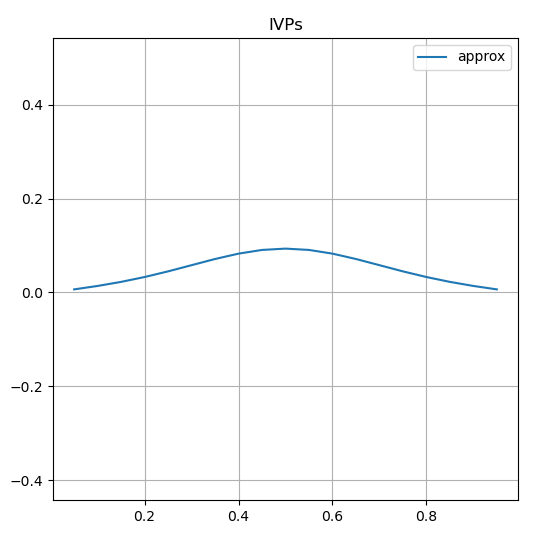
\includegraphics[width=0.2\textwidth]{BE10.png}
    \caption{BTCS method}
\end{figure}

\textbf{collocation method}
只需直接复用11章作业的配点法代码求解即可，得结果如下。
\begin{figure}[H]
    \centering
    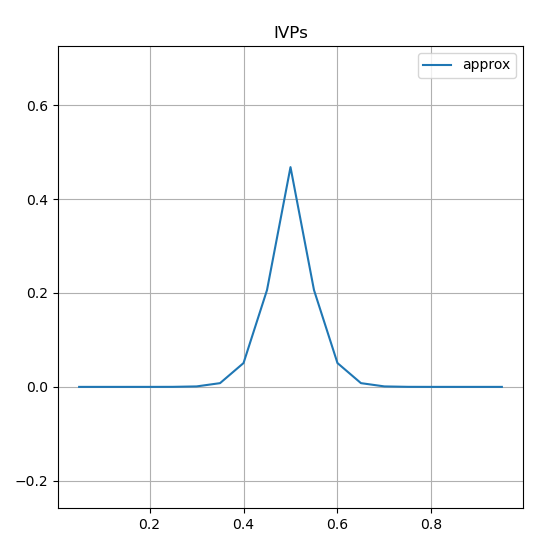
\includegraphics[width=0.2\textwidth]{Col1.png}
    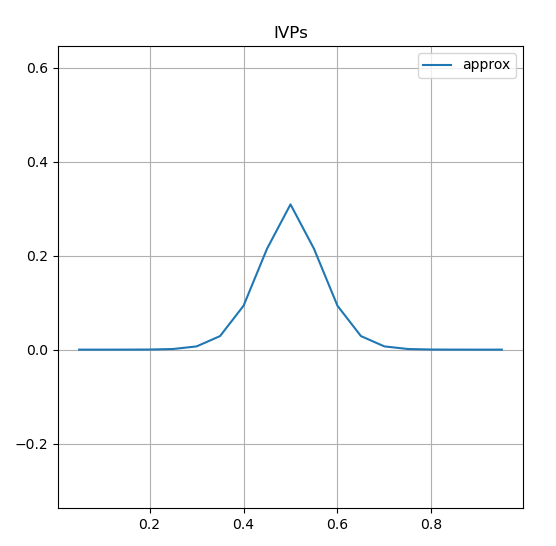
\includegraphics[width=0.2\textwidth]{Col2.png}
    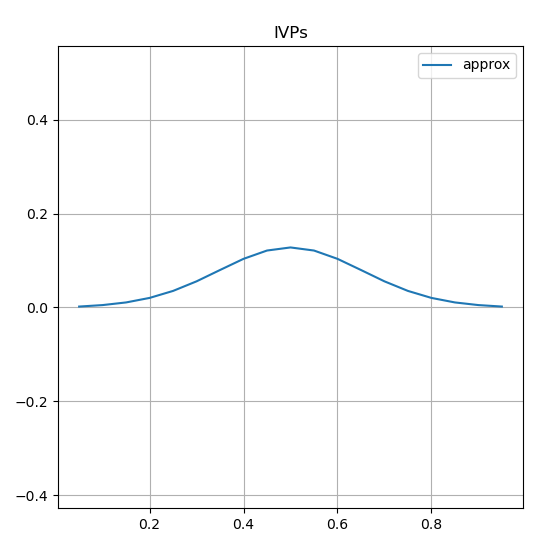
\includegraphics[width=0.2\textwidth]{Col10.png}
    \caption{collocation method}
\end{figure}

\textbf{FTCS}
因为向前欧拉法的必须要k<0.0015才能稳定，且$r = \frac{k}{h^2}$且$h = \frac{1}{20}$,
因此要想稳定必须r<0.5,以下是r=0.4的结果：
\begin{figure}[H]
    \centering
    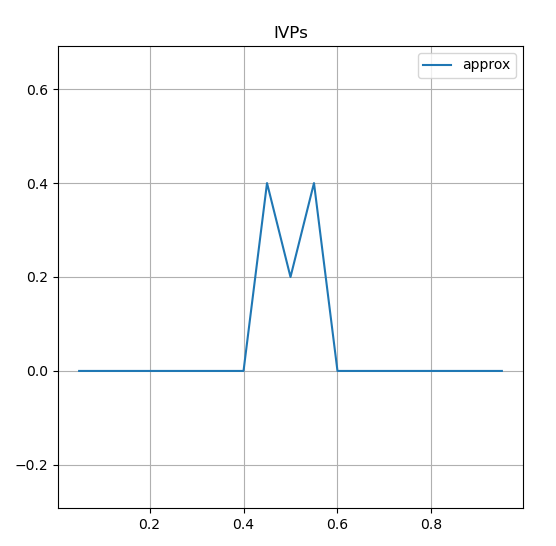
\includegraphics[width=0.2\textwidth]{FE1.png}
    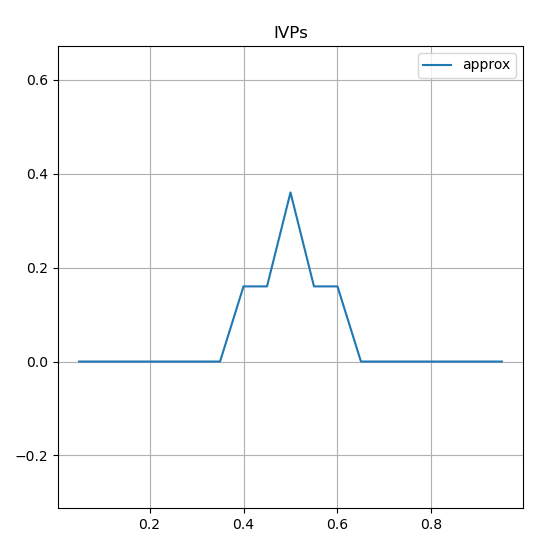
\includegraphics[width=0.2\textwidth]{FE2.png}
    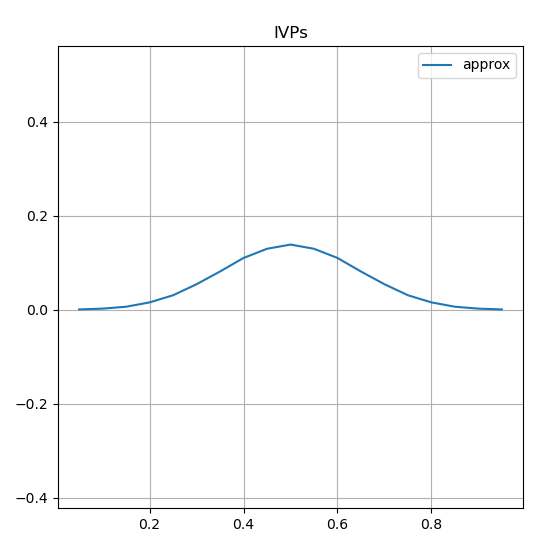
\includegraphics[width=0.2\textwidth]{FE10.png}
    \caption{FTCS method}
\end{figure}

% ===============================================

\end{document}